\documentclass[12pt,a4paper]{article}

%%%%%%%%%%%%%%%%%%%%%%%%% packages %%%%%%%%%%%%%%%%%%%%%%%%
\usepackage{tikz}
\usepackage{verbatim}
\usetikzlibrary{arrows,shapes}
\usepackage{amsmath}
\usepackage{amssymb}
\usepackage{physics}
\usepackage{amsthm}
\usepackage{amsmath}
\usepackage{amsfonts}
\usepackage{graphicx}
\usepackage[all]{xy}
\usepackage{tikz}
\usepackage{verbatim}
\usepackage[left=2cm,right=2cm,top=3cm,bottom=2.5cm]{geometry}
\usepackage{hyperref}
\usepackage{caption}
\usepackage{subcaption}
\usepackage{psfrag}

%%%%%%%%%%%%%%%%%%%%% students data %%%%%%%%%%%%%%%%%%%%%%%%
\newcommand{\student}{Your full name here!}
\newcommand{\course}{Course name goes here!}
\newcommand{\assignment}{Put a number here!}

%%%%%%%%%%%%%%%%%%% using theorem style %%%%%%%%%%%%%%%%%%%%

\newtheorem{thm}{Theorem}
\newtheorem{lem}[thm]{Lemma}
\newtheorem{defn}[thm]{Definition}
\newtheorem{exa}[thm]{Example}
\newtheorem{rem}[thm]{Remark}
\usepackage{braket}
\newtheorem{coro}[thm]{Corollary}
\newtheorem{quest}{Question}[section]

%%%%%%%%%%%%%%  Shortcut for usual set of numbers  %%%%%%%%%%%

\newcommand{\N}{\mathbb{N}}
\newcommand{\Z}{\mathbb{Z}}
\newcommand{\Q}{\mathbb{Q}}
\newcommand{\R}{\mathbb{R}}
\newcommand{\C}{\mathbb{C}}
\newcommand{\tens}[1]{%
	\mathbin{\mathop{\otimes}\limits_{#1}}%
}

%%%%%%%%%%%%%%%%%%%%%%%%%%%%%%%%%%%%%%%%%%%%%%%%%%%%%%%555
\begin{document}
\pgfdeclarelayer{background}
\pgfsetlayers{background,main}


%%%%%%%%%%%%%%%%%%%%%%% title page %%%%%%%%%%%%%%%%%%%%%%%%%%
\thispagestyle{empty}
\begin{center}
\textbf{AFRICAN INSTITUTE FOR MATHEMATICAL SCIENCES \\[0.5cm]
(AIMS RWANDA, KIGALI)}
\vspace{1.0cm}
\end{center}

%%%%%%%%%%%%%%%%%%%%% assignment information %%%%%%%%%%%%%%%%
\noindent
\rule{17cm}{0.2cm}\\[0.3cm]
Name: Sittana Osman Afifi Mohamedelmubarak \hfill  ch 3\\[0.1cm]
Zero Knowledge proof  \hfill Date: \today\\
\rule{17cm}{0.05cm}
\vspace{1.0cm}
%%%%%%%%%%%%%%%%%%%%%%%%%%%%%%%%%%%%%%%%%%%%%%%%%%%%%%%%%%%%%%%%%%%%%%%%%%%%%%%%%%\\
\\
In the previous chapter, we gave an introduction on Zero-knowledge proofs and Graph isomorphism based on zero-knowledge. In this chapter, we present an implementation of Graph isomorphisms based on zero-knowledge using Python for the original interaction between the prover and the verifier and for the simulator $S$ that we mentioned in chapter 2.\\
In addition, we show different scenarios for the prover and the verifier and examine the corresponding outputs.
According to our code, we suppose that the graphs we use are undirected and so the adjacency matrices are symmetric.
\section{Implementation}
According to the protocol that we discussed in the previous chapter, the input is two graphs and the output is a list containing:
$H=\sigma(G_0)$, $ch$, $\varphi$ and ’Accept’ or ’Reject’.
\subsection{Packages we import}
\begin{itemize}
	\item Math.
	\item Numpy.
	\item Graph-tools.
	\item Sympy.combinatorics.
	\item Csv.
	\item Networkx.
	\item Matplotlib.pyplot.
\end{itemize}
\subsection{Functions we use}
\begin{itemize}
	\item \textbf{generate-graph}\\
``generate-graph`` function enables us to transform the adjacency matrix into a graph using graph-tools package.
	\item \textbf{compose-permutation}\\
	``compose-permutation`` function lets us compose two permutations $(p,q)$ and return $p\circ q$.
	\item \textbf{apply-permute}\\
	``apply-permute`` function enables us to apply a permutation $P$ on adjacency matrix $AM$ and return another adjacency matrix $P(AM)$.
\item \textbf{inv}\\
``inv`` function takes a permutation $P$ as an input and returns the inverse of $P$ ($P^{-1}$). 
\item \textbf{are-equal}\\
``are-equal`` function checks if two adjacency matrices are equal or not.
\item \textbf{honest-prover}\\
``honest-prover`` function applies the protocol honestly for prover's side: It takes two adjacency matrices to represent two corresponding graphs $(G_0,G_1)$, the secret $\Pi$, seed $s$ to generate random permutation, and $mess-list$ as an output for the whole protocol to update it during interaction with the verifier. 
\item \textbf{honest-verifier}
``honest-verifier``  function applies the protocol honestly for the verifier's side: It takes two adjacency matrices to represent two corresponding graphs $(G_0,G_1)$, and $mess-list$ to update it during interaction with the prover. 
\item \textbf{graph-isomorphism}\\
``graph-isomorphism`` function enables us to run the protocol between the prover and the verifier by controlling the turn of each part.
\item \textbf{test-isomorphism}\\
``test-isomorphism`` function enables us to run ``graph-isomorpism`` by pass ``honest-prover`` and ``honest-verifier`` as a parameter to it.
\item \textbf{cheating-prover}\\
``cheating-prover`` function applies the protocol for cheating prover who doesn’t know the secret $\Pi$, it takes two adjacency matrices to represent two corresponding graphs $(G_0,G_1)$, seed $s$ to generate random permutation, and $mess-list$ as an output for the whole protocol to update it during interaction with the verifier.
\item \textbf{protocol-dishonest-prover}\\
``protocol-dishonest-prover`` function enables us to run ``graph-isomorpism`` by passing ``cheating-prover`` and ``honest-verifier`` as a parameter to it.
\item \textbf{simulator}\\
``simulator`` function enables us to applies the protocol for simulator $S$ that we mentioned in chapter 2.
\item \textbf{get-graph-from-file}\\
``get-graph-from-file`` lets us take a graph from csv file.
\item \textbf{get-pi-from-file}\\
``get-pi-from-file`` lets us take a secret $\Pi$ from csv file.
\item \textbf{equal}\\
``equal`` function is used after ``get-graph-from-file`` function to remove all additional data.
\item \textbf{plot-graph}\\
``plot-graph`` function uses networkx package to plot graphs using the corresponding adjacency matrix.
\end{itemize}
\subsection{Simulations and result}
In this section we show different scenarios and their results. Firstly Figure \ref{fig:csv} shows the csv file that contains our data:
\begin{figure}[h]
	\centering
	\includegraphics[width=1.15\linewidth]{csv}
	\caption{csv file}
	\label{fig:csv}
\end{figure}\\
We have four cases,  three of them using the original protocol and the last case using simulator, each one of them has two possible cases; which are \textbf{ch=0} (the fourth component is always Accept) and \textbf{ch=1}(the fourth component is different from one case to another):
\begin{itemize}
\item \textbf{Case 1: Interaction between honest prover and honest verifier}\\
First we get the adjacency matrices and $\Pi$ from a csv file and delete any additional data as follows:\\
\begin{figure}[h]
	\centering
	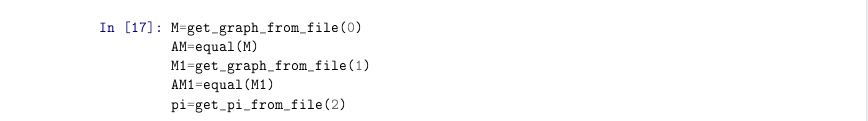
\includegraphics[width=1.25\linewidth]{3-1}
	\caption{Read the data from csv file}
	\label{fig:3-1}
\end{figure}\\
Then we plot $G_0$ and $G_1$, after that run the protocol when \textbf{ch=0} using code in Figure \ref{fig:3-2}:
\begin{figure}[h]
	\centering
	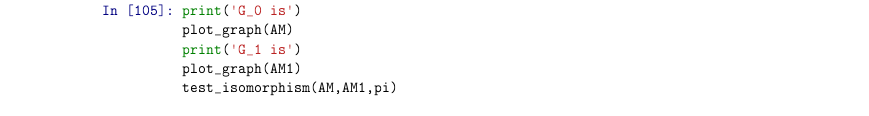
\includegraphics[width=1.25\linewidth]{3-2}
	\caption{Runing the protocol}
	\label{fig:3-2}
\end{figure}\\
The first output is printing the two graphs shown by Figure  \ref{fig:case 1,$G_0$ and $G_1$ with $ch=0$}:\\
\begin{figure}[h!]
	\centering\begin{subfigure}[b]{.4\linewidth}
		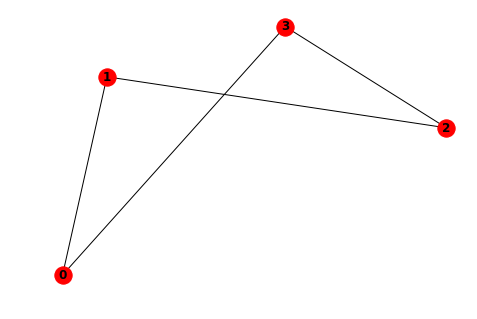
\includegraphics[width=\linewidth]{3-3.png}
		\caption{$G_0$.}
	\end{subfigure}
	\begin{subfigure}[b]{.4\linewidth}
		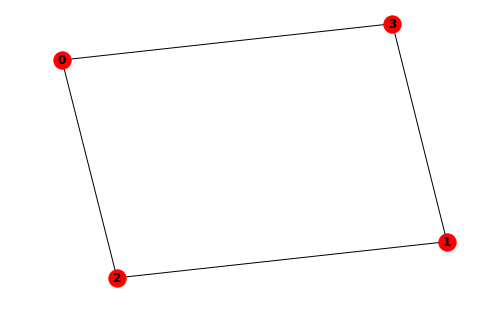
\includegraphics[width=\linewidth]{3-4.png}
		\caption{$G_1$.}
	\end{subfigure}
	\caption{$G_0$ and $G_1$ case 1 with $ch=0$}
	\label{fig:case 1,$G_0$ and $G_1$ with $ch=0$}
\end{figure}\\
Let us see the situation when the verifier chooses \textbf{ch=0}:\\
 \begin{figure}[h]
 	\centering
 	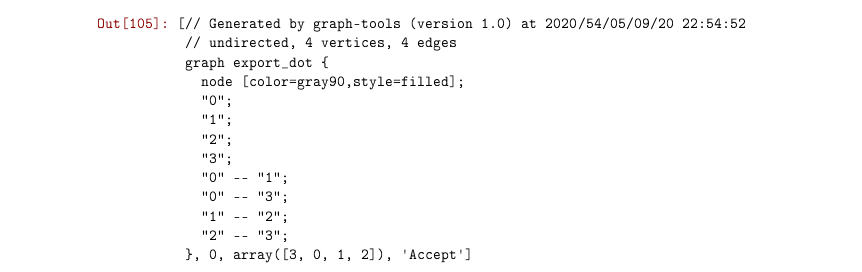
\includegraphics[width=1.25\linewidth]{3-5}
 	\caption{$mess-list$ when $ch=0$}
 	\label{fig:3-5}
 \end{figure}\\
As we mentioned earlier the fourth component is Accept.\\
For \textbf{ch=1}, the first output is printing the two graphs shown by Figure \ref{fig:case 1, $G_0$ and $G_1$ with $ch=1$}:
\begin{figure}[h!]
	\centering\begin{subfigure}[b]{.35\linewidth}
		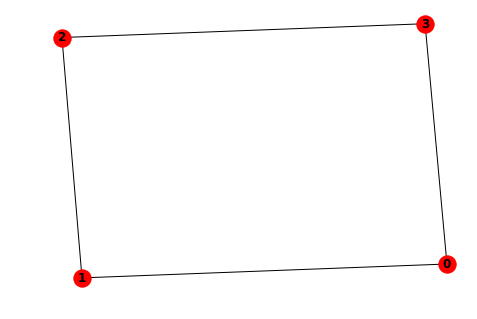
\includegraphics[width=\linewidth]{3-6.png}
		\caption{$G_0$.}
	\end{subfigure}
	\begin{subfigure}[b]{.35\linewidth}
		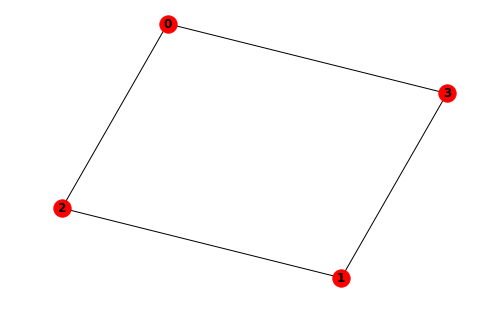
\includegraphics[width=\linewidth]{3-7.png}
		\caption{$G_1$.}
	\end{subfigure}
	\caption{case 1, $G_0$ and $G_1$ with $ch=1$}
	\label{fig:case 1, $G_0$ and $G_1$ with $ch=1$}
\end{figure}\\
Let us see the situation when the verifier chooses \textbf{ch=1}:\\
 \begin{figure}[h]
	\centering
	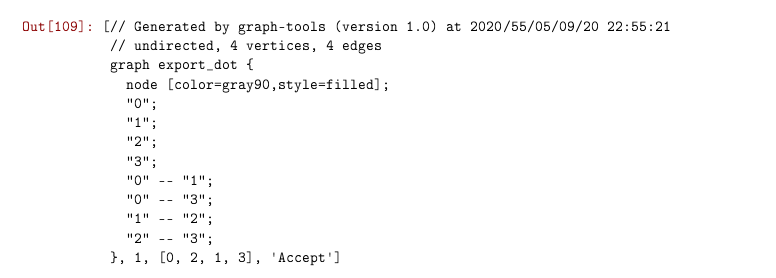
\includegraphics[width=1.25\linewidth]{3-8}
	\caption{$mess-list$ when $ch=1$}
	\label{fig:3-8}
\end{figure}\\
Since \textbf{ch=1} and the prover is honest, then the fourth element is Accept:\\
\item \textbf{Case 2: Interaction between cheating prover and honest verifier}\\
First, we update the second graph by reading it from csv file using code shown in Figure \ref{fig:3-9}:
\begin{figure}[h]
	\centering
	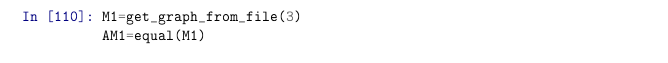
\includegraphics[width=1.25\linewidth]{3-9}
	\caption{Update the second graph}
	\label{fig:3-9}
\end{figure}\\
when \textbf{ch=0} the first output is printing the two graphs shown by Figure \ref{20}:\\
\begin{figure}[h!]
	\centering\begin{subfigure}[b]{.35\linewidth}
		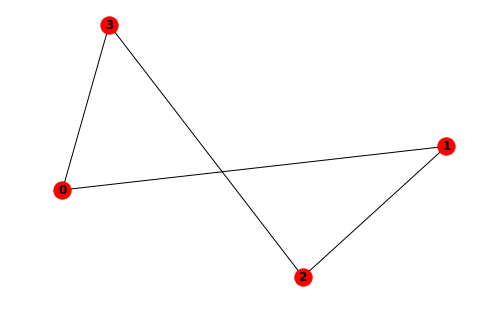
\includegraphics[width=\linewidth]{3-10.png}
		\caption{$G_0$.}
	\end{subfigure}
	\begin{subfigure}[b]{.35\linewidth}
		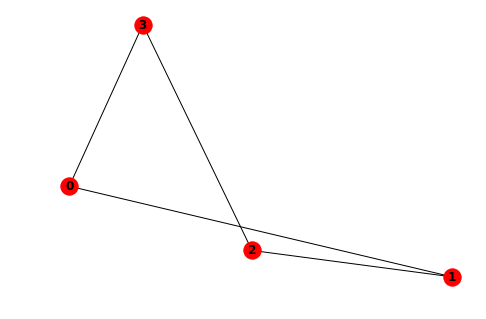
\includegraphics[width=\linewidth]{3-13.png}
		\caption{$G_1$.}
	\end{subfigure}
	\caption{case 2, $G_0$ and $G_1$ with $ch=0$}
	\label{20}
\end{figure}\\
Let us see the situation when the verifier chooses \textbf{ch=0}:\\
\begin{figure}[h]
	\centering
	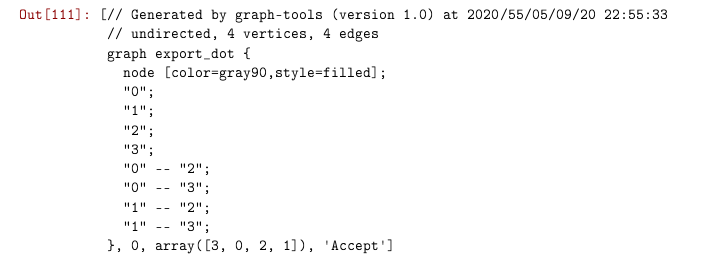
\includegraphics[width=1.25\linewidth]{3-12}
	\caption{$mess-list$ when $ch=0$}
	\label{fig:3-12}
\end{figure}\\
Since \textbf{ch=0} then the fourth component is always Accept even if the prover is dishonest.\\

When \textbf{ch=1}, the first output is the graph of $G_0$ and $G_1$ shown by Figure \ref{fig:$G_0$ and $G_1$ case 2 with $ch=1$}:\\
\begin{figure}[h!]
	\centering\begin{subfigure}[b]{.45\linewidth}
		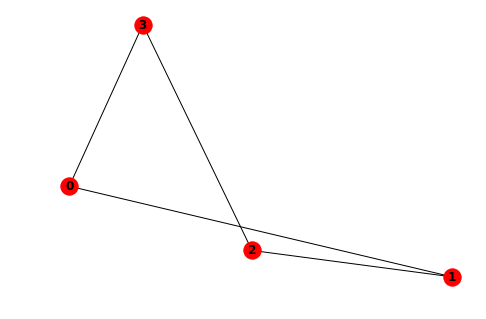
\includegraphics[width=\linewidth]{3-13.png}
		\caption{$G_0$.}
	\end{subfigure}
	\begin{subfigure}[b]{.45\linewidth}
		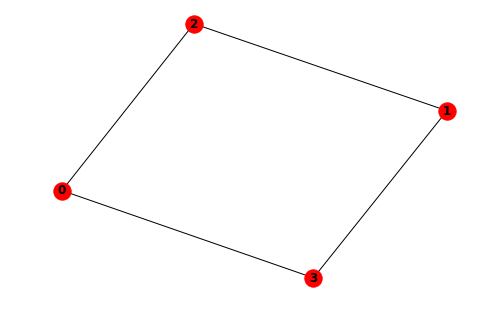
\includegraphics[width=\linewidth]{3-14.png}
		\caption{$G_1$.}
	\end{subfigure}
	\caption{$G_0$ and $G_1$ case 2 with $ch=1$}
	\label{fig:$G_0$ and $G_1$ case 2 with $ch=1$}
\end{figure}\\
The second output is $mess-list$, the last output is Reject because the prover is dishonest.
\item \textbf{Case 3: Interaction between honest prover and honest verifier for big graph (v=10,e=28)}\\
Now we apply ZKP for big isomorphic graphs that we can not check easily. First we read the data from the file using code shown by Figure \ref{fig:3-16}:\\
\\
\\
\begin{figure}[h]
	\centering
	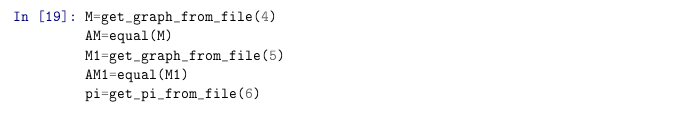
\includegraphics[width=0.95\linewidth]{3-16}
	\caption{updating data and run the protocol}
	\label{fig:3-16}
\end{figure}\\
With \textbf{ch=0}, the first output is the graph of $G_0$ and $G_1$ shown by Figure \ref{fig:case 3,$G_0$ and $G_1$, with $ch=0$}:\\
\begin{figure}[h!]
	\centering\begin{subfigure}[b]{.45\linewidth}
		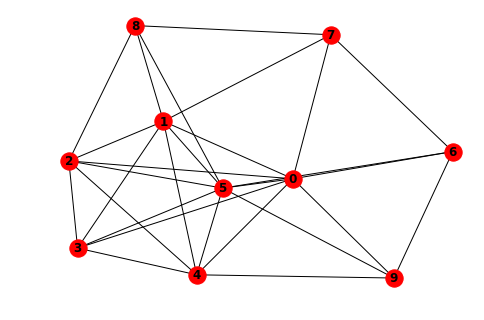
\includegraphics[width=\linewidth]{3-17.png}
		\caption{$G_0$.}
	\end{subfigure}
	\begin{subfigure}[b]{.45\linewidth}
		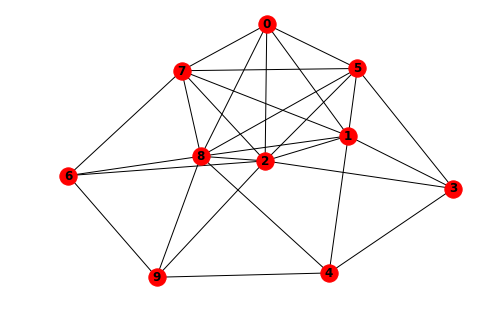
\includegraphics[width=\linewidth]{3-18.png}
		\caption{$G_1$.}
	\end{subfigure}
	\caption{case 3,$G_0$ and $G_1$, with $ch=0$}
	\label{fig:case 3,$G_0$ and $G_1$, with $ch=0$}
\end{figure}\\
The second output is $mess-lis$, and the fourth component when $ch=0$ is always Accept, Figure \ref{fig:3-19} shows the result:\\
\\
\\
\\
\\
\\
\\
\\
\\
\\
\\
\\
\\
\\
\\
\\
\\
\begin{figure}[h]
\centering
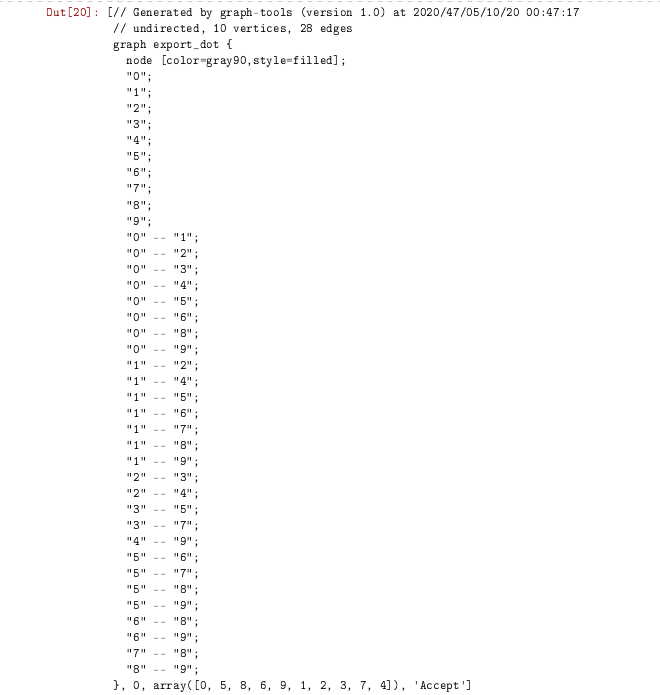
\includegraphics[width=0.85\linewidth]{3-19}
\caption{case 3 with $ch=0$}
\label{fig:3-19}
\end{figure}\\
 When \textbf{ch=1}, the first output is the graph of $G_0$ and $G_1$ shown by Figure \ref{fig:case 3,$G_0$ and $G_1$, with $ch=1$}:\\
 \begin{figure}[h!]
 	\centering\begin{subfigure}[b]{.35\linewidth}
 		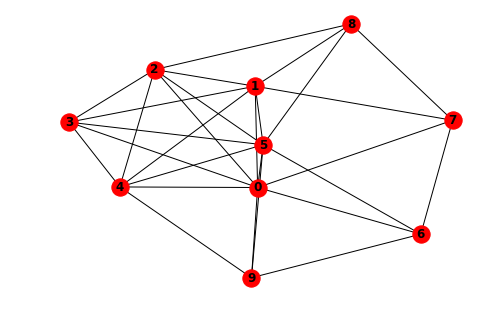
\includegraphics[width=\linewidth]{3-20.png}
 		\caption{$G_0$.}
 	\end{subfigure}
 	\begin{subfigure}[b]{.35\linewidth}
 		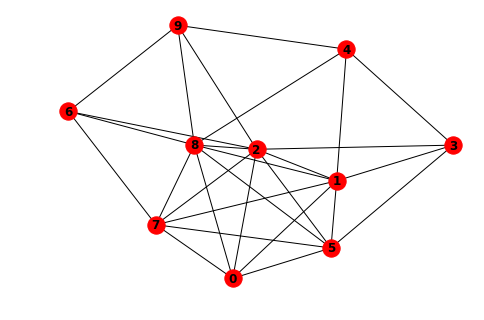
\includegraphics[width=\linewidth]{3-21.png}
 		\caption{$G_1$.}
 	\end{subfigure}
 	\caption{case 3,$G_0$ and $G_1$, with $ch=1$}
 	\label{fig:case 3,$G_0$ and $G_1$, with $ch=1$}
 \end{figure}\\
Let us see the situation when the verifier chooses \textbf{ch=1}, Figure \ref{fig:3-22} shows the result:\\
\begin{figure}[h]
	\centering
	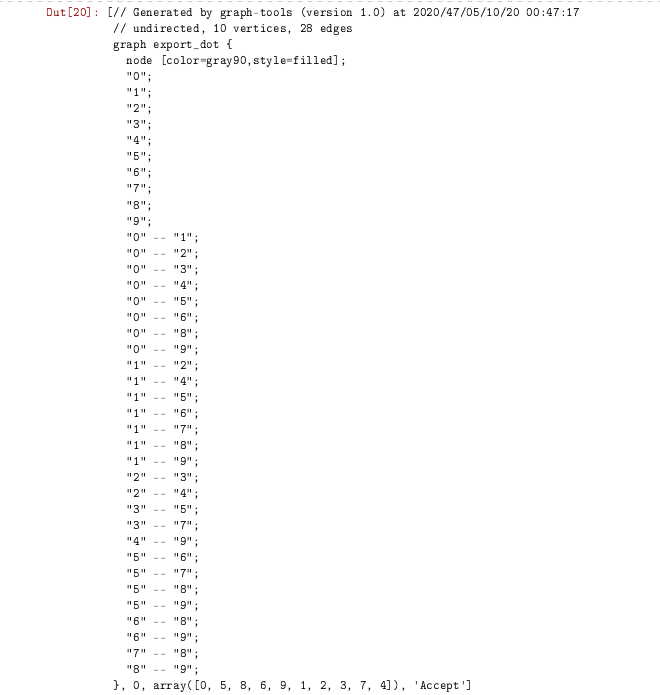
\includegraphics[width=0.95\linewidth]{3-19}
	\caption{$G_1$ case 3 with $ch=1$}
	\label{fig:3-22}
\end{figure}\\
\\
\item \textbf{Case 4: Interaction between cheating prover and honest verifier using simulator}\\
We use the same data in the previous case,so there is no need to update it,when $ch=0$ the first output is $G_0$ and $G_1$ shown by Figure \ref{fig: case 4, $G_0$ and $G_1$, with $ch=0$}:\\\\
\\
 \begin{figure}[h!]
	\centering\begin{subfigure}[b]{.45\linewidth}
		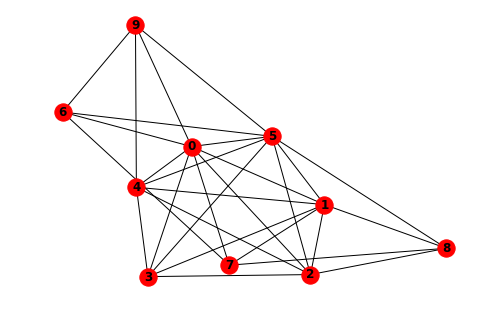
\includegraphics[width=\linewidth]{3-23.png}
		\caption{$G_0$.}
	\end{subfigure}
	\begin{subfigure}[b]{.45\linewidth}
		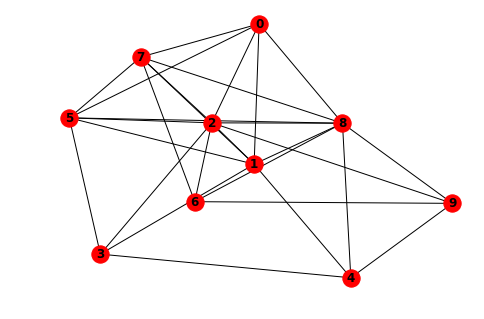
\includegraphics[width=\linewidth]{3-24.png}
		\caption{$G_1$.}
	\end{subfigure}
	\caption{ Case 4, $G_0$ and $G_1$ case 4 with $ch=0$}
	\label{fig: case 4, $G_0$ and $G_1$, with $ch=0$}
\end{figure}\\
The second output is $mess-list$, and the fourth component when $ch=0$ is Accept, Figure \ref{fig:3-25} shows the result:
\begin{figure}[h]
	\centering
	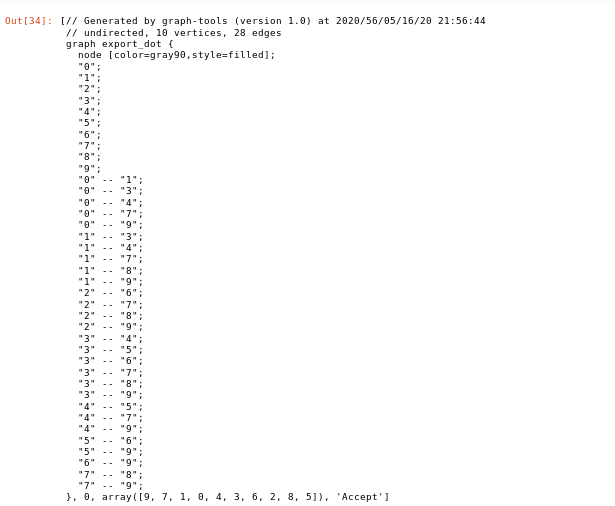
\includegraphics[width=0.7\linewidth]{3-25}
	\caption{case 4, $mess-list$ when $ch=0$}
	\label{fig:3-25}
\end{figure}\\
When $ch=1$ the first output is the graph of $G_0$ and $G_1$, shown by Figure \ref{fig:case 4,$G_0$ and $G_1$, with $ch=1$}:\\
\\
\\
\\
\\
\\
\begin{figure}[h!]
	\centering\begin{subfigure}[b]{.45\linewidth}
		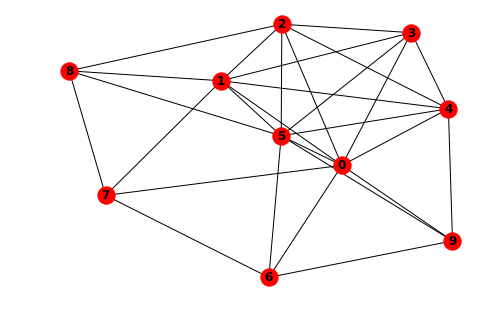
\includegraphics[width=\linewidth]{3-26.png}
		\caption{$G_0$.}
	\end{subfigure}
	\begin{subfigure}[b]{.45\linewidth}
		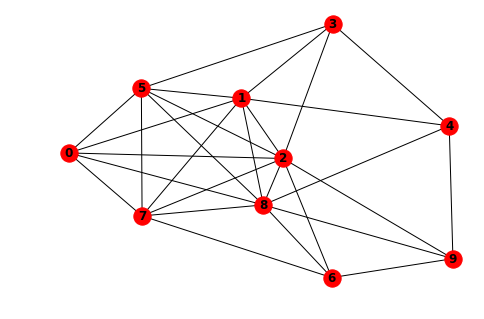
\includegraphics[width=\linewidth]{3-27.png}
		\caption{$G_1$.}
	\end{subfigure}
	\caption{Case 4, $G_0$ and $G_1$ with $ch=1$}
	\label{fig:case 4,$G_0$ and $G_1$, with $ch=1$}
\end{figure}\\
The second output is $mess-lis$, and the fourth component when $ch=1$ is Accept since the prover is honest, Figure \ref{fig:3-28} shows the result:\\
\begin{figure}[h]
	\centering
	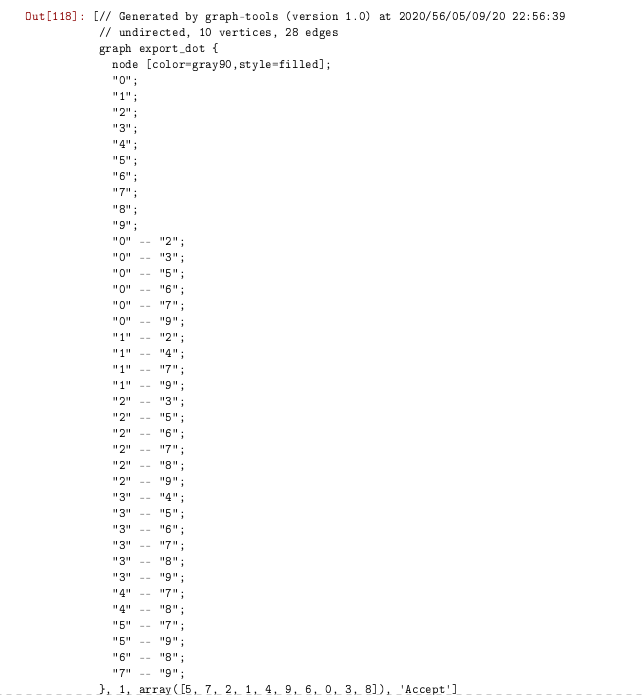
\includegraphics[width=0.95\linewidth]{3-28}
	\caption{$mess-list$ case 4 with $ch=1$}
	\label{fig:3-28}
\end{figure}\\
\end{itemize}

%\bibliography{refer}
%\bibliographystyle{ieeetr}
\end{document}